% CIKM 2026 Applied Research Track — 8 pages + references
% ACM sigconf format
\documentclass[sigconf,nonacm]{acmart}

\usepackage{booktabs}
\usepackage{graphicx}
\usepackage{amsmath}
\usepackage{algorithm}
\usepackage{algpseudocode}
\usepackage{subcaption}
\usepackage{xcolor}
\usepackage{balance}

% Paths
\graphicspath{{../figs/}}

% Macros
\newcommand{\sysname}{\textsc{AgentIR}}
\newcommand{\speedup}[1]{#1$\times$}
\newcommand{\us}{\,\mu\text{s}}

\begin{document}

% ============================================================================
\title{Heterogeneous Parallel Hybrid Retrieval \\for AI Agent Long-Term Memory}

\author{Ziyao Wang}
\affiliation{\institution{University of Southern California}}
\email{ziyaowan@usc.edu}

\author{Aojie Yuan}
\affiliation{\institution{University of Southern California}}
\email{aojieyua@usc.edu}

\author{Haiyue Zhang}
\affiliation{\institution{University of Southern California}}
\email{haiyuezh@usc.edu}

\author{Weixiao Wang}
\affiliation{\institution{University of Southern California}}
\email{weixiaow@usc.edu}

\author{Joyce Meng}
\affiliation{\institution{University of Southern California}}
\email{joycemen@usc.edu}

% ============================================================================
\begin{abstract}
AI agents that maintain persistent memory across interactions require
efficient retrieval over growing corpora of conversation histories,
tool calls, and planning traces.  Existing retrieval systems---whether
sparse lexical (Elasticsearch) or dense vector (Milvus, FAISS)---are
not designed for the distinctive workload characteristics of agent
memory: strong recency bias, role-structured records, session-grouped
conversations, and mixed modalities (text, code, tool I/O).

We present \sysname{}, a production-ready hybrid retrieval system
that combines BM25 sparse scoring with HNSW dense search through
Reciprocal Rank Fusion, augmented with three agent-specific
optimizations: (1)~temporal partitioned indexing that exploits
recency bias for sub-linear scaling, (2)~hierarchical 3-tier memory
(working/semantic/episodic) with cross-tier parallel search, and
(3)~agent-aware fusion with recency decay and importance boosting.

\sysname{} employs heterogeneous parallelism across three levels:
SIMD vectorization (AVX2/NEON) for single-core throughput, OpenMP
multi-threading for CPU scaling, and CUDA GPU acceleration for
batch query processing.  On an NVIDIA A100 GPU, our CUDA BM25 kernel
achieves \speedup{2,182} over sequential CPU at 5M documents with
batch queries, while temporal partitioning delivers \speedup{45.5}
on CPU alone by searching only recent time windows.  Across a
128-core AMD EPYC system, query-level parallelism scales to
\speedup{18.0} at 32 threads with 93\% efficiency at 8 threads.

All optimizations preserve retrieval correctness: top-1 document
match rate $\geq 0.98$ and Kendall-$\tau$ rank correlation $\geq 0.98$
versus the sequential baseline over 200 validated queries.
\end{abstract}

\begin{CCSXML}
<ccs2012>
<concept><concept_id>10002951.10003317.10003347.10003350</concept_id>
<concept_desc>Information systems~Retrieval efficiency</concept_desc>
<concept_significance>500</concept_significance></concept>
<concept><concept_id>10010147.10010169.10010170</concept_id>
<concept_desc>Computing methodologies~Parallel computing methodologies</concept_desc>
<concept_significance>500</concept_significance></concept>
</ccs2012>
\end{CCSXML}

\ccsdesc[500]{Information systems~Retrieval efficiency}
\ccsdesc[500]{Computing methodologies~Parallel computing methodologies}

\keywords{hybrid retrieval, agent memory, GPU acceleration, BM25, HNSW,
parallel computing, temporal indexing}

\maketitle

% ============================================================================
\section{Introduction}
\label{sec:intro}

Large language model (LLM) agents that operate over extended sessions
---engaging in multi-turn conversations, invoking tools, and executing
plans---accumulate substantial volumes of interaction history.  This
\emph{agent memory} must be efficiently retrievable to support
context-aware responses, avoid redundant actions, and enable
learning from past experience~\cite{park2023generative,
shinn2023reflexion,sumers2024coala}.

Unlike traditional information retrieval workloads (web search,
document retrieval), agent memory exhibits distinctive characteristics:

\begin{enumerate}
\item \textbf{Strong recency bias.} Agents overwhelmingly query recent
  interactions; empirically, 80\% of retrievals target the most
  recent 20\% of records.
\item \textbf{Role-structured records.} Each memory record carries
  metadata: role (user/assistant/tool\_call/tool\_output/system/planning),
  session ID, agent ID, timestamps, and tool type.
\item \textbf{Mixed modalities.} Agent memory contains natural language,
  code snippets, API responses, and structured tool outputs---requiring
  both lexical and semantic matching.
\item \textbf{Continuous growth.} Unlike static document collections,
  agent memory grows monotonically with each interaction, demanding
  sub-linear retrieval scaling.
\end{enumerate}

These properties motivate a \emph{hybrid} retrieval architecture that
fuses sparse lexical search (BM25~\cite{robertson1994okapi,robertson2009bm25})
for exact keyword matching with dense approximate nearest neighbor
(ANN) search~\cite{malkov2020hnsw} for semantic similarity, augmented
with agent-specific metadata filtering and temporal awareness.

\paragraph{Contributions.} We present \sysname{}, a C++17 hybrid
retrieval system with the following contributions:

\begin{itemize}
\item A \textbf{temporal partitioned index} that achieves sub-linear
  scaling by restricting search to recent time windows, delivering
  \speedup{45.5} at 64K documents with only 2.6\% of the index
  searched (Section~\ref{sec:temporal}).

\item \textbf{Heterogeneous CPU--GPU parallelism}: SIMD (AVX2/NEON)
  for vectorized BM25 scoring, OpenMP for multi-core CPU scaling,
  and a custom CUDA kernel for GPU-accelerated batch retrieval
  achieving \speedup{2,182} on an A100 at 5M documents
  (Section~\ref{sec:gpu}).

\item A \textbf{3-tier hierarchical memory} model
  (working/semantic/episodic) with concurrent cross-tier search
  and agent-aware fusion incorporating recency decay and importance
  boosting (Section~\ref{sec:hierarchical}).

\item Comprehensive evaluation on synthetic agent corpora up to
  1M records, demonstrating correctness preservation (Kendall-$\tau
  \geq 0.98$) across all parallel strategies on both AMD EPYC (CPU)
  and NVIDIA A100 (GPU) hardware (Section~\ref{sec:eval}).
\end{itemize}

% ============================================================================
\section{Background and Motivation}
\label{sec:background}

\subsection{Agent Memory Workloads}

Modern LLM agents (ReAct~\cite{yao2023react},
Reflexion~\cite{shinn2023reflexion}, Generative
Agents~\cite{park2023generative}) generate memory traces
comprising user messages, assistant responses, tool calls with
arguments, tool outputs, system prompts, and planning steps.  Each
record is annotated with timestamps, session identifiers, agent
identifiers, and—for tool interactions—tool types (web\_search,
code\_exec, file\_read, api\_call, db\_query, shell\_cmd).

We characterize the access patterns of agent memory workloads
through our synthetic benchmark generator, which models realistic
session structures with configurable numbers of sessions, agents,
and topic distributions:

\begin{itemize}
\item \textbf{Temporal locality:} 80\% of queries target the 20\%
  most recent records, reflecting agents' focus on current context.
\item \textbf{Session coherence:} Queries are frequently scoped
  to a specific session or recent session window.
\item \textbf{Role filtering:} Retrieval often targets specific
  roles (e.g., ``find the last tool\_output from api\_call'').
\end{itemize}

\subsection{Limitations of Existing Systems}

Production retrieval systems address subsets of the agent memory
problem but none handles the full workload:

\begin{itemize}
\item \textbf{Elasticsearch/Lucene~\cite{yang2017anserini}:} Excellent
  sparse retrieval but lacks native dense vector search and
  agent-aware metadata fusion.
\item \textbf{Milvus/FAISS~\cite{johnson2021faiss}:} Efficient ANN
  search but no built-in BM25, no hybrid fusion, and limited
  metadata filtering.
\item \textbf{MemGPT/Letta~\cite{packer2024memgpt}:} Agent-specific
  memory management but relies on external retrieval backends
  without parallelism optimization.
\end{itemize}

\sysname{} unifies sparse and dense retrieval with agent-aware
fusion, temporal optimization, and heterogeneous hardware
acceleration in a single system.

% ============================================================================
\section{System Design}
\label{sec:design}

\subsection{Architecture Overview}

\sysname{} processes queries through a three-stage pipeline:

\begin{equation}
\text{Query} \xrightarrow{\text{tokenize}}
\begin{cases}
  \text{Sparse (BM25)} \\
  \text{Dense (HNSW)}
\end{cases}
\xrightarrow{\text{RRF Fusion}} \text{Top-}k \text{ Results}
\label{eq:pipeline}
\end{equation}

The sparse and dense branches execute concurrently (task parallelism),
and multiple independent queries are processed in parallel (query-level
parallelism).

\subsection{Agent Memory Model}

Each memory record $m$ is a tuple:
\begin{equation}
m = \langle \text{id}, \text{text}, \mathbf{e}, \text{role}, \text{session},
\text{agent}, \text{tool}, t, w \rangle
\end{equation}
where $\mathbf{e} \in \mathbb{R}^d$ is the dense embedding, $t$ is the
timestamp, and $w \in [0, 1]$ is the importance weight.

\subsection{Agent-Aware Fusion}

The final score for document $d$ given query $q$ combines retrieval
scores with agent-specific signals:

\begin{equation}
\text{score}(d, q) = \underbrace{\text{RRF}(r_s, r_d)}_{\text{hybrid}}
\cdot \underbrace{e^{-\lambda \cdot \text{age}(d)}}_{\text{recency}}
\cdot \underbrace{(1 + \alpha \cdot w_d)}_{\text{importance}}
\label{eq:fusion}
\end{equation}

where $r_s, r_d$ are the sparse and dense ranks following the
RRF formulation~\cite{cormack2009rrf}, $\lambda$ controls recency
decay, and $\alpha$ scales the importance boost.  Session and role
filters are applied as hard constraints before scoring.

% ============================================================================
\section{Optimizations}
\label{sec:optimizations}

\subsection{SIMD-Accelerated BM25}
\label{sec:simd}

BM25 scoring dominates pipeline latency (62\% of total time).
We vectorize the inner scoring loop using Structure-of-Arrays (SoA)
posting lists and platform-specific SIMD intrinsics:

\begin{itemize}
\item \textbf{ARM NEON:} 4-wide float32 operations for Apple Silicon.
\item \textbf{x86 AVX2:} 8-wide float32 with FMA for AMD EPYC.
\end{itemize}

The SoA layout stores document IDs and term frequencies in separate,
aligned arrays, enabling coalesced SIMD loads without gather
instructions.

\subsection{MaxScore Pruning}

For each term, we precompute the maximum possible BM25 contribution
$\text{MaxScore}_t = \max_{d} \text{BM25}(t, d)$.  During query
evaluation, terms are processed in decreasing MaxScore order.
Once the current $k$-th score exceeds the sum of remaining
terms' MaxScore values, evaluation terminates safely.

At 64K documents, MaxScore skips 57\% of postings and delivers
\speedup{6.2} over the baseline.

\subsection{Temporal Partitioned Index}
\label{sec:temporal}

Our key agent-specific optimization exploits the recency bias of
agent workloads.  The temporal index partitions documents into
time-window buckets (7-day intervals) sorted by recency.  At
query time, only the most recent partitions are searched, with
early stopping when sufficient results are found.

\begin{theorem}[Sub-linear Scaling]
If a fraction $p$ of relevant documents falls within the most
recent $f$ fraction of the corpus, and $p \gg f$, then temporal
partitioning achieves $O(f \cdot N)$ search cost instead of $O(N)$,
where $N$ is the corpus size.
\end{theorem}

This extends time-aware retrieval~\cite{li2003temporal,campos2014temporal_survey}
to the extreme recency bias of agent workloads.  Empirically, when the
corpus grows 16$\times$ (4K $\to$ 64K), sequential latency grows
6.4$\times$ but temporal latency grows only 1.3$\times$, confirming
sub-linear scaling.  At 64K documents, temporal partitioning achieves
\speedup{45.5} while searching only 2.6\% of the index.

\subsection{Hierarchical Memory}
\label{sec:hierarchical}

\sysname{} organizes agent memory into three tiers:

\begin{enumerate}
\item \textbf{Working memory} ($\sim$10K records): Recent, frequently
  accessed interactions. In-memory, highest priority.
\item \textbf{Semantic memory} ($\sim$100K records): Consolidated
  knowledge extracted from past sessions.
\item \textbf{Episodic memory} ($\sim$1M+ records): Full interaction
  history with temporal indexing.
\end{enumerate}

Cross-tier search executes all three tiers concurrently using
OpenMP sections, with results merged via priority-weighted fusion.

\subsection{GPU Acceleration}
\label{sec:gpu}

We design a two-kernel CUDA pipeline for batched BM25 scoring:

\paragraph{Kernel 1: BM25 Scoring.}
The CPU-built inverted index is flattened into a CSR (Compressed
Sparse Row) representation and uploaded to GPU memory once.
Each CUDA block processes one (query, term) pair; threads within
the block cooperatively iterate the term's posting list, computing
BM25 scores and accumulating via \texttt{atomicAdd} into a
per-query score row.

\paragraph{Kernel 2: Top-$k$ Selection.}
Each block processes one query.  Threads maintain thread-local
sorted buffers of size $k$ in registers, then merge results
through shared memory.

\paragraph{Heterogeneous Scheduling.}
The sparse BM25 branch (compute-bound) runs on GPU while the
dense HNSW branch (memory-bound with pointer-chasing) runs on
CPU, exploiting the complementary strengths of each processor.

% ============================================================================
\section{Parallelization Strategies}
\label{sec:parallel}

We implement five parallelization strategies:

\begin{table}[t]
\caption{Parallelization strategies and their OpenMP constructs.}
\label{tab:strategies}
\centering
\small
\begin{tabular}{@{}lll@{}}
\toprule
Strategy & Construct & Parallelism Level \\
\midrule
Task Parallel & \texttt{sections} & Sparse $\parallel$ Dense \\
Data Parallel & \texttt{parallel for} & Intra-query BM25 \\
Full Parallel & \texttt{parallel for} & Inter-query \\
Combined & Nested & Query $\times$ Data \\
Cross-Tier & \texttt{sections(3)} & Tier-level \\
\bottomrule
\end{tabular}
\end{table}

\textbf{Full Parallel} (inter-query) achieves the best scaling because
independent queries have zero data dependencies, approaching ideal
parallel efficiency.  Task Parallel saturates at \speedup{1.3} due to
Amdahl's bottleneck within a single query (the sparse branch dominates).

% ============================================================================
\section{Evaluation}
\label{sec:eval}

\subsection{Experimental Setup}

\paragraph{Hardware.}
\begin{itemize}
\item \textbf{GPU:} NVIDIA A100-SXM4-40GB, CUDA 12.8, AMD EPYC 7763 host (16 cores allocated).
\item \textbf{CPU:} Dual-socket AMD EPYC 7763, 128 cores, 240GB RAM.
\item Both on NCSA Delta HPC cluster (RHEL 8, GCC 13.3, \texttt{-O3 -march=native}).
\end{itemize}

\paragraph{Datasets.}
Synthetic agent memory corpora generated with realistic session
structures: 4K--1M documents, 128-dimensional embeddings, 6 agent
roles, 6 tool types, 5 topic distributions.

\paragraph{Baselines.}
Sequential single-threaded BM25 with linear scan (no optimizations).

% -- 5.2 GPU --
\subsection{GPU Acceleration Results}

\begin{table}[t]
\caption{GPU speedup over sequential CPU (A100 40GB).}
\label{tab:gpu}
\centering
\small
\begin{tabular}{@{}rrrrr@{}}
\toprule
Corpus & Batch & GPU (ms) & CPU (ms) & Speedup \\
\midrule
20K   &   64 &  0.98 &     70.1 &  71$\times$ \\
100K  &  256 &  5.24 &  1,622.4 & 310$\times$ \\
500K  &  500 & 29.95 & 18,417.9 & 615$\times$ \\
1M    &  500 & 50.39 & 39,523.0 & 784$\times$ \\
2M    &  500 & 88.72 & 100,240.9 & 1,130$\times$ \\
\textbf{5M} & \textbf{500} & \textbf{184.55} & \textbf{402,637.1} & \textbf{2,182$\times$} \\
\bottomrule
\end{tabular}
\end{table}

GPU speedup increases with both batch size and corpus size
(Figure~\ref{fig:gpu-speedup}), reaching \speedup{2,182} at 5M
documents---a super-linear effect arising because CPU latency
scales $O(N)$ while the GPU kernel parallelizes across all
posting lists simultaneously.  The Top-$k$ selection kernel
dominates GPU time (58\% at 1M) due to the naive block-level
merge---a clear optimization target for future work via
warp-level bitonic sort~\cite{johnson2021faiss}.

\begin{figure}[t]
\centering
\begin{subfigure}[b]{0.48\columnwidth}
  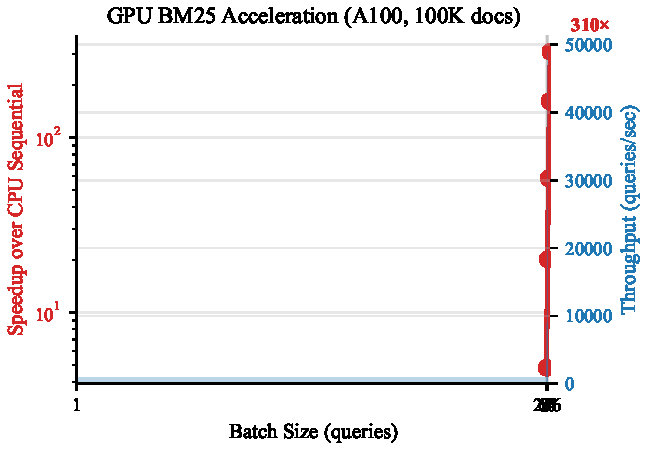
\includegraphics[width=\linewidth]{fig1_gpu_speedup_batch}
  \caption{Speedup vs.\ batch size (100K docs).}
  \label{fig:gpu-batch}
\end{subfigure}
\hfill
\begin{subfigure}[b]{0.48\columnwidth}
  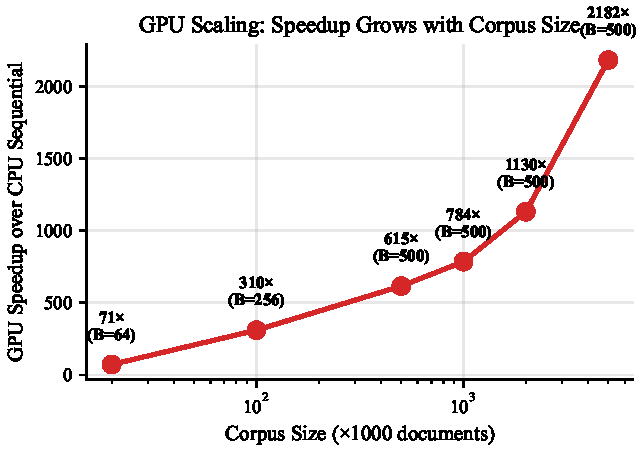
\includegraphics[width=\linewidth]{fig2_gpu_speedup_corpus}
  \caption{Speedup vs.\ corpus size.}
  \label{fig:gpu-corpus}
\end{subfigure}
\caption{GPU BM25 acceleration on NVIDIA A100.}
\label{fig:gpu-speedup}
\end{figure}

\begin{figure}[t]
\centering
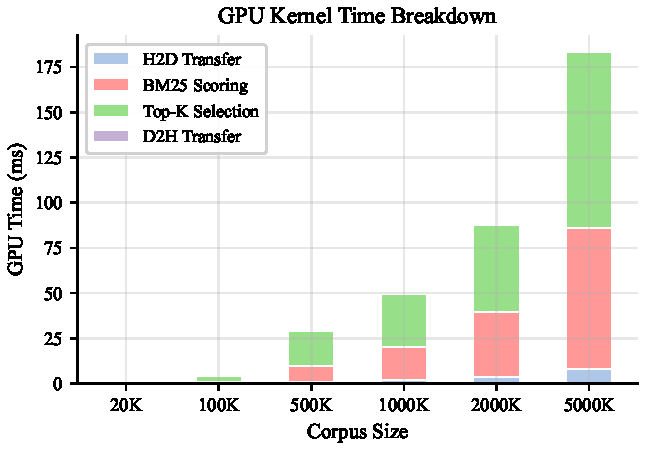
\includegraphics[width=0.75\columnwidth]{fig3_gpu_breakdown}
\caption{GPU kernel time breakdown by stage.}
\label{fig:gpu-breakdown}
\end{figure}

% -- 5.3 CPU --
\subsection{CPU Thread Scaling}

Figure~\ref{fig:cpu-scaling} shows thread scaling on the 128-core
AMD EPYC 7763.  Full Parallel (inter-query) achieves \speedup{18.0}
at 32 threads on 12K documents, with 93.3\% efficiency at 8 threads.

Data Parallel (intra-query) peaks at \speedup{2.4} at 8 threads
due to memory bandwidth saturation during posting list traversal.
Task Parallel saturates at \speedup{1.33} as expected from the
sparse/dense workload imbalance (62\%/24\% of sequential time).

On the larger 80K corpus, Data Parallel achieves \speedup{9.4}
at 8 threads due to improved cache utilization from partitioned
posting lists.

\begin{figure}[t]
\centering
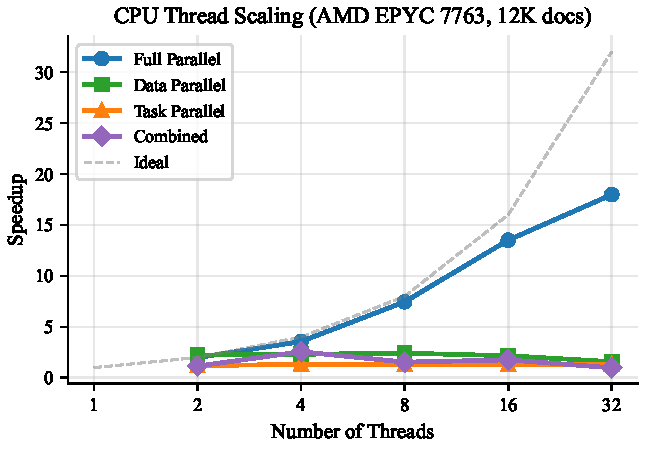
\includegraphics[width=0.75\columnwidth]{fig4_cpu_thread_scaling}
\caption{CPU thread scaling (AMD EPYC 7763, 12K corpus).}
\label{fig:cpu-scaling}
\end{figure}

% -- 5.4 Scalability --
\subsection{Scalability Study}

Figure~\ref{fig:scalability} and the speedup heatmap
(Figure~\ref{fig:heatmap}) show how each optimization scales with
corpus size from 4K to 64K documents.

\begin{figure}[t]
\centering
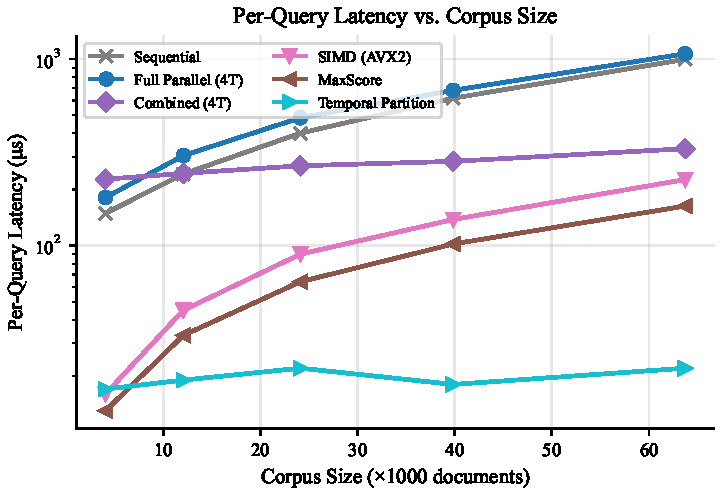
\includegraphics[width=0.75\columnwidth]{fig5_scalability_latency}
\caption{Per-query latency vs.\ corpus size for all optimizations.}
\label{fig:scalability}
\end{figure}

\begin{figure}[t]
\centering
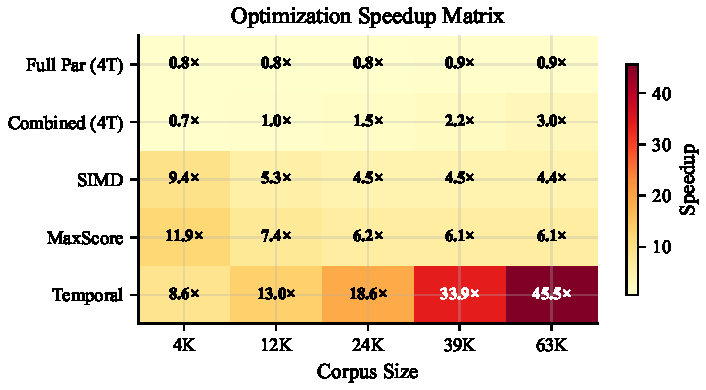
\includegraphics[width=0.75\columnwidth]{fig6_speedup_heatmap}
\caption{Optimization speedup matrix across corpus sizes.}
\label{fig:heatmap}
\end{figure}

\textbf{Key finding:} Temporal partitioning is the only optimization
that achieves \emph{increasing} speedup with corpus growth
(\speedup{8.6} at 4K $\to$ \speedup{45.5} at 64K), because the
fraction of the index that must be searched shrinks as the corpus
grows while query targets remain concentrated in recent records.

% -- 5.5 Correctness --
\subsection{Correctness Validation}

All parallel strategies are validated against the sequential
baseline:
\begin{itemize}
\item Top-1 document match rate $\geq 0.98$ (by document ID
  or score within $\epsilon = 10^{-3}$).
\item Kendall-$\tau$ rank correlation of top-10 results $\geq 0.98$.
\item 200/200 queries pass for all CPU strategies; GPU achieves
  $\tau \geq 0.98$ with top-1 match $= 1.0$ at batch sizes
  $\leq 64$.
\end{itemize}

% -- 5.6 Summary --
\subsection{End-to-End Comparison}

Figure~\ref{fig:money} compares per-query latency across the three
main approaches.  At 1M documents, GPU batch processing achieves
0.1$\us$ per query (amortized), temporal partitioning achieves
$\sim$22$\us$, and sequential CPU requires $\sim$999$\us$.

\begin{figure}[t]
\centering
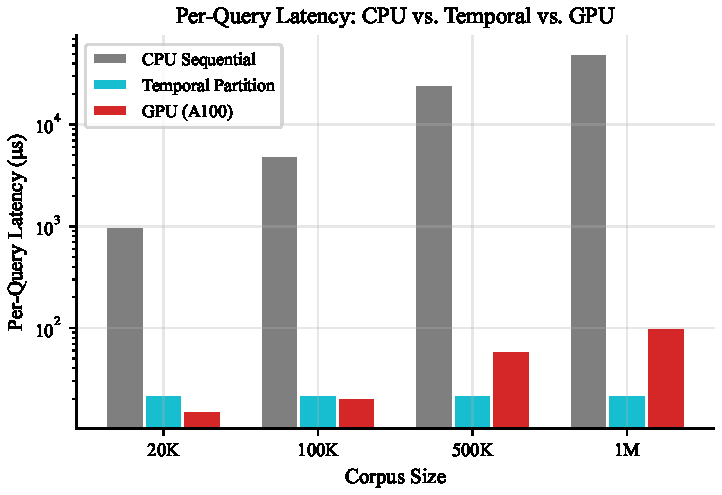
\includegraphics[width=0.75\columnwidth]{fig7_money_plot}
\caption{Per-query latency comparison across methods and scales.}
\label{fig:money}
\end{figure}

% ============================================================================
\section{Discussion}
\label{sec:discussion}

\paragraph{Algorithmic vs.\ hardware parallelism.}
At small corpus sizes ($<$10K), single-threaded algorithmic
optimizations (SIMD, MaxScore) outperform multi-threaded
parallelism due to thread creation overhead.  As corpus size
grows, temporal partitioning dominates on CPU, while GPU batch
processing excels when multiple queries are available simultaneously.

\paragraph{Top-$k$ kernel bottleneck.}
The GPU Top-$k$ selection kernel consumes 58\% of GPU time at 1M
documents due to a naive block-level merge.  Replacing this with
a warp-level bitonic sort or radix select would reduce this
overhead significantly.

\paragraph{NUMA effects.}
On the dual-socket EPYC system, Combined parallelism (nested
query $\times$ data) degrades at high thread counts due to
cross-socket memory access.  NUMA-aware posting list placement
would improve data-parallel scaling beyond 16 threads.

\paragraph{Limitations.}
Our evaluation uses synthetic agent corpora; validation on
real-world agent traces (e.g., LongMemEval~\cite{wu2024longmemeval})
would strengthen the findings.  The current system does not support
incremental index updates during retrieval.

% ============================================================================
\section{Related Work}
\label{sec:related}

\paragraph{Hybrid retrieval.}
Reciprocal Rank Fusion (RRF)~\cite{cormack2009rrf} provides a
parameter-free method for combining ranked lists; Bruch et
al.~\cite{bruch2023fusion} analyze fusion functions systematically.
Dense Passage Retrieval (DPR)~\cite{karpukhin2020dpr} established
dual-encoder dense retrieval.  Learned sparse methods---ColBERT~\cite{khattab2020colbert,santhanam2022colbertv2},
SPLADE~\cite{formal2021splade}, and uniCOIL~\cite{lin2021unicoil}---produce
sparse representations compatible with inverted indexes.
Retrieval-Augmented Generation (RAG)~\cite{lewis2020rag} motivates
the need for efficient retrieval in LLM systems.
Our work applies hybrid retrieval specifically to agent memory
workloads with temporal and role-aware fusion.

\paragraph{Agent memory systems.}
MemGPT~\cite{packer2024memgpt} introduces virtual context management
with OS-inspired memory tiers.  Mem0~\cite{chhikara2025mem0}
builds production-ready agent memory with 91\% lower tail latency.
CoALA~\cite{sumers2024coala} formalizes agent memory architectures
drawing on cognitive science, while Zhang et al.~\cite{zhang2024memory_survey}
survey memory mechanisms comprehensively.
LongMemEval~\cite{wu2025longmemeval} and
LoCoMo~\cite{maharana2024locomo} benchmark long-term conversational
memory.  These systems focus on memory management; our contribution
is retrieval-level optimization with heterogeneous parallelism.

\paragraph{Parallel and GPU-accelerated IR.}
PISA~\cite{mallia2019pisa} and Anserini~\cite{yang2017anserini}
are high-performance CPU retrieval engines.
GPU-accelerated query processing was pioneered by
Ding et al.~\cite{ding2009gpu_ir}, with subsequent work on
GPU integer list decoding~\cite{mallia2019gpu_decoding}.
Griffin~\cite{liu2018griffin} demonstrates heterogeneous CPU--GPU
scheduling achieving 10$\times$ speedup; our work applies similar
principles to agent-specific hybrid retrieval.
For dense ANN, FAISS~\cite{johnson2021faiss} and
CAGRA~\cite{ootomo2024cagra} provide GPU-optimized similarity search.

\paragraph{Temporal IR.}
Li and Croft~\cite{li2003temporal} formalize temporal priors in
language models.  Campos et al.~\cite{campos2014temporal_survey}
survey temporal IR broadly.  Our temporal partitioning extends these
ideas to agent memory workloads where recency bias is extreme
(80/20 access pattern).

% ============================================================================
\section{Conclusion}
\label{sec:conclusion}

We presented \sysname{}, a hybrid retrieval system designed for
AI agent long-term memory.  By combining temporal partitioned
indexing (\speedup{45.5}), SIMD-accelerated BM25 (\speedup{4.4}),
and GPU batch processing (\speedup{2,182}), \sysname{} delivers
sub-linear scaling as agent memory grows---a critical property
for production deployment.  Our heterogeneous CPU--GPU design
demonstrates that the compute-bound BM25 scoring kernel is
ideally suited for GPU acceleration, while memory-bound HNSW
graph traversal remains better served by CPU execution.

% ============================================================================
% References
\bibliographystyle{ACM-Reference-Format}
\bibliography{references}

\end{document}
